\documentclass[12pt]{article}
\usepackage{graphicx}
\usepackage{float}
\usepackage{amsmath}
\usepackage{amscd}
\usepackage{hyperref}
\usepackage{enumerate}
\usepackage{amsfonts}
\usepackage{amssymb}
\usepackage[utf8]{inputenc}
\usepackage{amsthm}
\usepackage{subcaption}
\usepackage{listings}
\usepackage{tikz}
\usepackage{color} %red, green, blue, yellow, cyan, magenta, black, white
\usepackage{fullpage}
\usepackage{mathtools}
\usepackage{booktabs}
\usepackage{longtable}

\definecolor{mygreen}{RGB}{28,172,0} % color values Red, Green, Blue
\definecolor{mylilas}{RGB}{170,55,241}

\newtheorem{theorem}{Teorema}
\newtheorem{lem}[theorem]{Lemma}
\newtheorem{dfn}{Definición}
\newtheorem{cor}[theorem]{Corolario}
\newtheorem{obs}{Obs}
\newtheorem{rem}{Remark}
\newtheorem{prob}{Problema}

\newcommand*\circled[1]{\tikz[baseline=(char.base)]{
            \node[shape=circle,draw,inner sep=.05pt] (char) {#1};}}
            


\newtheoremstyle{named}{}{}{\itshape}{}{\bfseries}{.}{.5em} {\thmnote{#3 }#1}
\theoremstyle{named}
\newtheorem*{namedtheorem}{}



\newcounter{exercisecounter}
\newenvironment{ex}{\begin{quote}%
    \refstepcounter{exercisecounter}%
  \textbf{Ejercicio \arabic{exercisecounter}}%
  \quad
}{%
\end{quote}%
}
\newcounter{ejemplocounter}
\newenvironment{ej}{\begin{quote}%
    \refstepcounter{ejemplocounter}%
  \textbf{Ejemplo \arabic{ejemplocounter}}%
  \quad
}{%
\end{quote}%
}

\renewcommand{\d}[1]{\ensuremath{\operatorname{d}\!{#1}}}

\DeclarePairedDelimiter{\ceil}{\lceil}{\rceil}


\newcommand{\folder}{./Effect}

\begin{document}


\title{Treatment effects}

\author{Instituto Tecnológico Autónomo de México}
\date{\today}
\maketitle


\hrulefill


\section{\Huge{Some Summary Statistics}}

\vspace{7mm}

\subsection*{Administrative Stats}

Summary statistics of basic subject characteristics. All variables coming from casefile details are tested for balance between survey and non-survey populations.

\begin{center}
\scriptsize{
\begin{table}[!htbp] \centering 
  \caption{} 
  \label{} 
\begin{tabular}{@{\extracolsep{5pt}} cccccccc} 
\\[-1.8ex]\hline 
\hline \\[-1.8ex] 
Statistic & Treatment & Control & Treatment.1 & Control.1 & t-stat & Treatment.2 & Control.2 \\ 
\hline \\[-1.8ex] 
Wage & $1,522$ & $396$ & $620.698$ & $580.082$ & $0.797$ & $787.098$ & $930.839$ \\ 
Female & $1,522$ & $396$ & $0.445$ & $0.444$ & $0.013$ & $0.497$ & $0.498$ \\ 
Public Lawyer & $1,522$ & $396$ & $0.064$ & $0.071$ & $$-$0.486$ & $0.244$ & $0.257$ \\ 
Tenure & $1,522$ & $396$ & $3.898$ & $4.073$ & $$-$0.555$ & $5.299$ & $5.668$ \\ 
Bought durable goods recently & $170$ & $25$ & $0.082$ & $0.080$ & $$ & $0.276$ & $0.277$ \\ 
Working at the time & $172$ & $24$ & $0.465$ & $0.458$ & $$ & $0.500$ & $0.509$ \\ 
Looking for a job & $168$ & $24$ & $0.571$ & $0.500$ & $$ & $0.496$ & $0.511$ \\ 
\hline \\[-1.8ex] 
\end{tabular} 
\end{table} 
}
\end{center}

\pagebreak

\subsection*{Expectation Stats}

Summary statistics for expectations.

\begin{center}
\scriptsize{
\begin{table}[!htbp] \centering 
  \caption{} 
  \label{} 
\begin{tabular}{@{\extracolsep{5pt}}lccccc} 
\\[-1.8ex]\hline 
\hline \\[-1.8ex] 
Statistic & \multicolumn{1}{c}{N} & \multicolumn{1}{c}{Mean} & \multicolumn{1}{c}{St. Dev.} & \multicolumn{1}{c}{Min} & \multicolumn{1}{c}{Max} \\ 
\hline \\[-1.8ex] 
Payment prob. (baseline) & 248 & 78.782 & 24.885 & 10 & 100 \\ 
Payment amount (baseline) & 210 & 69,297.190 & 104,987.700 & 0.000 & 850,000.000 \\ 
Payment prob. (exit) & 186 & 70.452 & 28.466 & 10 & 100 \\ 
Payment amount (exit) & 157 & 58,355.640 & 73,370.290 & 0.000 & 500,000.000 \\ 
\hline \\[-1.8ex] 
\end{tabular} 
\end{table} 
}
\end{center}

\pagebreak

\subsection*{Update in beliefs}

The update in beliefs is measured in relative terms, this is the percentage deviation of the exit survey with respect to the entrance survey
\[\frac{exit-initial}{initial}\]

We provide two measures: Update in beliefs in probability and payment.\\

\begin{center}
\scriptsize{
\begin{table}[htbp]\centering \caption{Update in beleifs \label{sumstat}}
\begin{tabular}{l c c c c c}\hline\hline
\multicolumn{1}{c}{\textbf{Variable}} & \textbf{Mean}
 & \textbf{Std. Dev.}& \textbf{Min.} &  \textbf{Max.} & \textbf{N}\\ \hline
update\_emp\_fir\_law & -0.026 & 1.171 & -1 & 9 & 180\\
update\_emp & -0.106 & 0.578 & -1 & 2.2 & 70\\
update\_emp\_law & -0.216 & 0.560 & -1 & 1.875 & 210\\
\hline\end{tabular}
\end{table}
}
\end{center}

\begin{figure}[H]
\label{diff}
\begin{center}
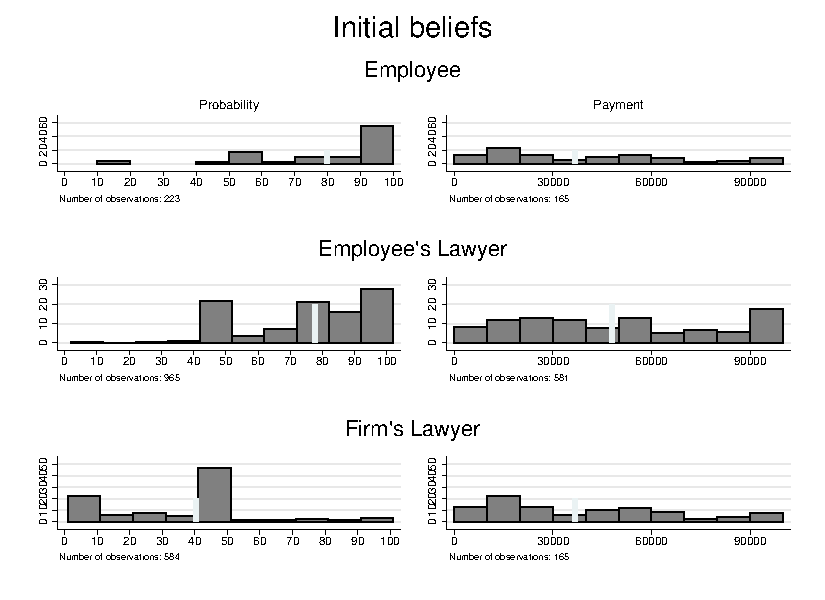
\includegraphics[width=\textwidth]{./Figures/belief.pdf}
\end{center}
{\footnotesize \textit{The histograms are trimmed at the 90 percentile in the case for amount. Width of bins are \$50,000 pesos for the case of amount and 10\% for the case of probability.}}
\end{figure}


\begin{figure}[H]
\label{update}
\begin{center}
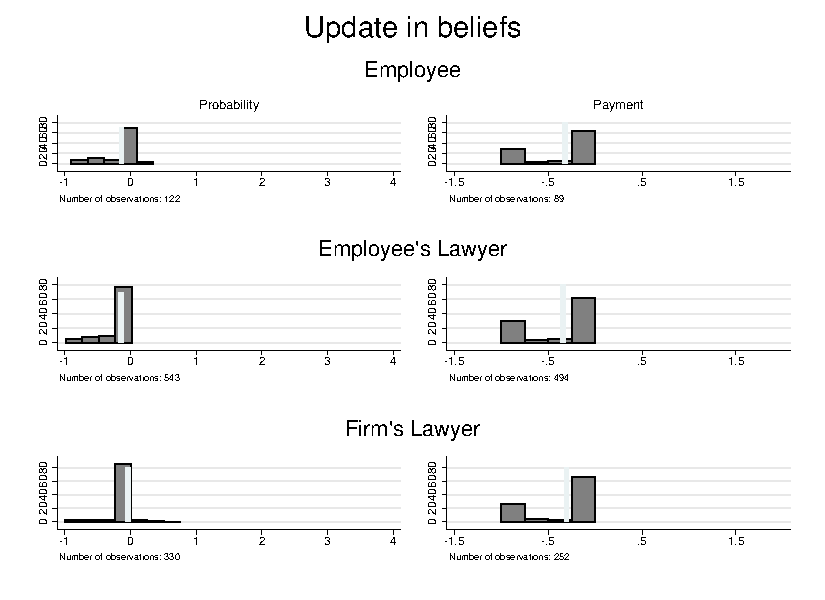
\includegraphics[width=\textwidth]{./Figures/update_belief.pdf}
\end{center}
{\footnotesize \textit{The histograms measures the update in relative terms. Width of bins is 0.25 }}
\end{figure}

\pagebreak

Now we test difference in initial and exit survey in expectations. The following table shows the results.

\begin{center}
\scriptsize{% Table generated by Excel2LaTeX from sheet 'ttest'
\begin{tabular}{rrrr}
\toprule
      & \multicolumn{1}{c}{Initial} & \multicolumn{1}{c}{Exit} & \multicolumn{1}{c}{p-value} \\
\midrule
\multicolumn{4}{c}{Probability} \\
\midrule
\midrule
Employee  & \multicolumn{1}{l}{79.927} & \multicolumn{1}{l}{71.945} & \multicolumn{1}{l}{0} \\
      & \multicolumn{1}{l}{(24.703)} & \multicolumn{1}{l}{(28.661)} & \multicolumn{1}{l}{} \\
Employees Lawyer & \multicolumn{1}{l}{77.007} & \multicolumn{1}{l}{67.658} & \multicolumn{1}{l}{0} \\
      & \multicolumn{1}{l}{(20.208)} & \multicolumn{1}{l}{(24.383)} & \multicolumn{1}{l}{} \\
Firms Lawyer & \multicolumn{1}{l}{40.822} & \multicolumn{1}{l}{42.267} & \multicolumn{1}{l}{0.122} \\
      & \multicolumn{1}{l}{(23.101)} & \multicolumn{1}{l}{(23.24)} & \multicolumn{1}{l}{} \\
      \midrule
\multicolumn{4}{c}{Payment levels} \\
\midrule
\midrule
Employee  & \multicolumn{1}{l}{54344.478} & \multicolumn{1}{l}{54930.941} & \multicolumn{1}{l}{0.804} \\
      & \multicolumn{1}{l}{(64865.672)} & \multicolumn{1}{l}{(66475.18)} & \multicolumn{1}{l}{} \\
Employees Lawyer & \multicolumn{1}{l}{97829.594} & \multicolumn{1}{l}{88209.612} & \multicolumn{1}{l}{0} \\
      & \multicolumn{1}{l}{(108525.677)} & \multicolumn{1}{l}{(97808.871)} & \multicolumn{1}{l}{} \\
Firms Lawyer & \multicolumn{1}{l}{56229.145} & \multicolumn{1}{l}{54309.441} & \multicolumn{1}{l}{0.564} \\
      & \multicolumn{1}{l}{(74573.935)} & \multicolumn{1}{l}{(67685.482)} & \multicolumn{1}{l}{} \\
      \midrule
\multicolumn{4}{c}{Payment logs} \\
\midrule
\midrule
Employee  & \multicolumn{1}{l}{10.219} & \multicolumn{1}{l}{10.269} & \multicolumn{1}{l}{0.454} \\
      & \multicolumn{1}{l}{(1.709)} & \multicolumn{1}{l}{(1.617)} & \multicolumn{1}{l}{} \\
Employees Lawyer & \multicolumn{1}{l}{10.855} & \multicolumn{1}{l}{10.771} & \multicolumn{1}{l}{0.002} \\
      & \multicolumn{1}{l}{(1.569)} & \multicolumn{1}{l}{(1.523)} & \multicolumn{1}{l}{} \\
Firms Lawyer & \multicolumn{1}{l}{9.422} & \multicolumn{1}{l}{9.483} & \multicolumn{1}{l}{0.554} \\
      & \multicolumn{1}{l}{(3.303)} & \multicolumn{1}{l}{(3.117)} & \multicolumn{1}{l}{} \\
\bottomrule
\end{tabular}%
}
\end{center}


%%%%%%%%%%%%%%%%%%%%%%%%%%%%%%%%%%%%%%%%%%%%%%%%%%%%%%%%%%%%%%%%%%%%%%%%%%%%%%%%
\end{document}
